Our experimental results in \S\ref{sec:results} highlight why \textit{compression} is essential to make our approach work.
%
We used ParLOT to record a unique 16-bit identifier for every function call and return.
%
Tracing just this small amount of information without compression when running the Mantevo miniapps~\cite{mantevo} on Stampede 1 resulted in about 2 MB/s of data per core on average.
%
Extrapolating this value to all 102,400 cores of Stampede 1 (not counting the accelerators) yields 205 GB/s of trace data, which exceeds the Lustre filesystem's parallel write performance of 150 GB/s.
%
Enabling ParLOT's compression algorithm reduced the emitted trace data by a factor of 100 on average, a ratio that is quite stable w.r.t scaling, making it possible to trace full-scale programs while leaving over 98\% of the I/O bandwidth to the application. Therefore, ParLOT should also work for codes with higher requirement bandwidth than the ones we tested.

Figure \ref{overview} provides a general overview of \parlot 's workflow.
%
Basic blocks within program executables are {\em dynamically} instrumented before being executed and collected data getting compressed on-the-fly during runtime. 
%

\begin{figure}[!t]
\centering
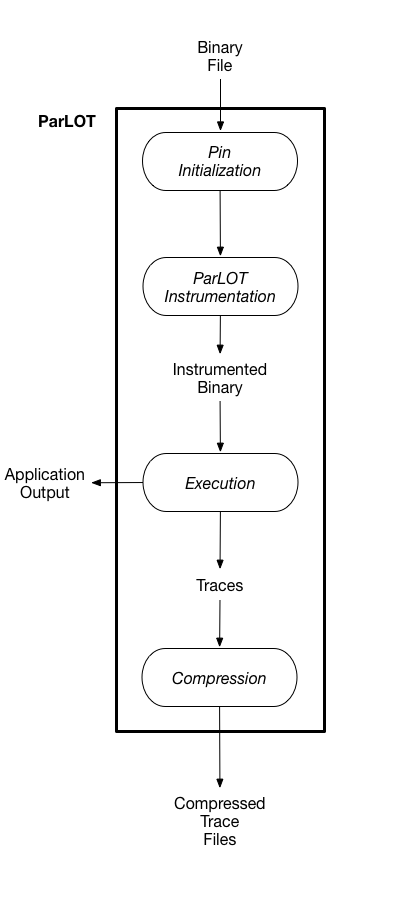
\includegraphics[width=1.75in]{overview.png}
\caption{Overview of \parlot}
\label{overview}
\end{figure}


\subsection{Tracing Operation}
\label{subsec:traceOp}

\parlot uses the PIN API as its instrumentation mechanism to gather traces. In particular, it instructs \pin to instrument every thread launch and termination in the application as well as every function entry and exit. The thread-launch instrumentation code initializes the per-thread tracing variables and opens a file into which the trace data from that thread will be written. The thread-termination code finalizes any ongoing compression, flushes out any remaining entries, and closes the trace file. \parlot assigns every static function in each image (main program and all libraries) a unique unsigned 16-bit ID, which it records in a separate file together with the image and function name. This file allows the trace reader to map IDs back to function-name/image pairs.

For every function \emph{entry}, \parlot executes extra code that has access to the thread ID, function ID, and current stack-pointer (SP) value. Based on the SP value, it performs call-stack correction if necessary (see \S\ref{subsec:stack_cor}), adds the new function to a data structure it maintains that holds the call stack (which is separate from the application's runtime stack), and emits the function ID into the trace file via an incremental compression algorithm (see \S\ref{subsec:incr-compr}). All of this is done independently for each thread. Similarly, for every function \emph{exit}, \parlot also executes extra code that has access to the thread ID, function ID, and current SP value. Based on the SP value, it performs call-stack correction if necessary, removes the function from its call-stack data structure, and emits the reserved function ID of zero into the trace file to indicate an exit. As before, this is done via an incremental compression algorithm. We use zero for all exits rather than emitting the function ID and a bit to specify whether it is an entry or exit because using zeros results in more compressible output. This way, half of the values in the trace will be zero.





\subsection{Incremental Compression}
\label{subsec:incr-compr}

\parlot immediately compresses the traced information even before it is written to memory. It does, however, keep a sliding window (circular buffer) of the most recent uncompressed trace events, which is needed by the compressor. It compresses each function ID before the next function ID is known. The conventional approach would be to first record uncompressed function IDs in a buffer and later compress the whole buffer once it fills up. However, this makes the processing time very non-uniform. Whereas almost all function IDs can be recorded very quickly since they just have to be written to the buffer, processing a function ID that happens to fill the buffer takes a long time as it triggers the compression of the entire buffer. This results in sporadic blocking of threads during which time they make no progress towards executing the application code. Initial experiments revealed that such behavior can be detrimental when one thread is polling data from another thread that is currently blocked due to compression. For example, we observed a several order of magnitude increase in entry/exit events of an internal MPI library function when using block-based compression.

To remedy this situation, the compressor must operate incrementally, i.e., each piece of trace data must be compressed when it is generated, without buffering it first, to ensure that there is never a long-latency compression delay. Few existing compression algorithms have been implemented in such a manner because it is more difficult to code up and probably a little slower. Nevertheless, we were able to implement our algorithm (discussed next) in this way so that each trace event is compressed with similar latency.


\subsection{Compression Algorithm}
\label{subsec:compAlg}

We used the CRUSHER framework~\cite{mb-cluster15, mb-space16, mb-sc16, mb-dcc18} to automatically synthesize an effective and fast lossless compression algorithm for our traces. CRUSHER is based on a library of data transformations extracted from various compression algorithms. It combines these transformations in all possible ways to generate algorithm candidates, which it then evaluates on a set of training data. We gathered uncompressed traces from some of the Mantevo miniapps~\cite{mantevo} for this purpose. This evaluation revealed that a particular word-level Lempel-Ziv (LZ) transformation followed by a byte-level Zero-Elimination (ZE) transformation works well. In other words, \parlot 's trace entries, which are two-byte words, are first transformed using LZ. The output is interpreted as a sequence of bytes, which is transformed using ZE for further compression. The output of ZE is written to secondary storage.

LZ implements a variant of the LZ77 algorithm~\cite{LZ}. It uses a 4096-entry hash table to identify the most recent prior occurrence of the current value in the trace. Then it checks whether the three values immediately before that location match the three trace entries just before the current location. If they do not, the current trace entry is emitted and LZ advances to the next entry. If the three values match, LZ counts how many values following the current value match the values following that location. The length of the matching substring is emitted and LZ advances by that many values. Note that all of this is done incrementally. The history of previous trace entries available to LZ for finding matches is maintained in a 64k-entry circular buffer. 

ZE emits a bitmap in which each bit represents one input byte. The bits indicate whether the corresponding bytes are zero or not. Following each eight-bit bitmap, ZE emits the non-zero bytes.

As mentioned above, we had to implement the two transformations incrementally to minimize the latency. This required breaking them up into multiple pieces. Depending on the state the compressor is in when the next trace entry needs to be processed, the appropriate piece of code is executed and the state updated. If the LZ code produces an output, which it only does some of the time, then the appropriate piece of the ZE code is executed in a similar manner.


\subsection{\pin and Call-Stack Correction}
\label{subsec:stack_cor}

To be able to decode the trace, i.e., to correctly associate each exit with the function entry it belongs to, our trace reader maintains an identical call-stack data structure. Unfortunately, and as pointed out in the \pin documentation~\cite{pinurl}, it is not always possible to identify all function exits. For example, in optimized code, a function's instructions may be inlined and interleaved with the caller's instructions, making it sometimes infeasible for \pin to identify the exit. As a consequence, we have to ensure that \parlot works correctly even when \pin misses an exit. This is why the SP values are needed.

During tracing, \parlot not only records the function IDs in its call stack but also the associated SP values. This enables it to detect missing exits and to correct the call stack accordingly. Whenever a function is entered, it checks if there is at least one entry in the call stack and, if so, whether its SP value is higher than that of the current SP. If it is lower, we must have missed at least one exit since the runtime stack grows downwards (the SP value decreases with every function entry and increases with every exit). If a missing exit is detected in this manner, \parlot pops the top element from its call stack and emits a zero to indicate a function exit. It repeats this procedure until the stack is empty or its top entry has a sufficiently high SP value. The same call-stack correction technique is applied for every function exit whose SP value is inconsistent. Note that the SP values are only used for this purpose and are not included in the compressed trace.

The result is an internally consistent trace of function entry and exit events, meaning that parsing the trace will yield a correct call stack. This is essential so that the trace can be decoded properly. Moreover, it means that the trace includes exits that truly happened in the application but that were missed by \pin. Note, however, that our call-stack correction is a best-effort approach and may, in rare cases, temporarily not reflect what the application actually did. For example, this can happen for functions that do not create a frame on the runtime stack. When implementing \parlot on top of another DBI framework, call-stack correction may not be needed, resulting in even lower \parlot overhead.
